\documentclass[a4paper]{ctexart}
\usepackage[top=2.3cm,bottom=2cm,left=1.7cm,right=1.7cm]{geometry} 
\usepackage{amsmath} 
\usepackage{booktabs}
\usepackage{amsthm}
\usepackage{longtable} 
\usepackage{graphicx}
\usepackage{subfigure}
\usepackage{caption}
\usepackage{fontspec}
\usepackage{titlesec}
\usepackage{fancyhdr}
\title{\textbf{测定非线性元件的伏安特性}}
\author{王崇斌 1800011716}
\date{}
\makeatletter %使\section中的内容左对齐
\renewcommand{\section}{\@startsection{section}{1}{0mm}
	{-\baselineskip}{0.5\baselineskip}{\bf\leftline}}
\makeatother
\begin{document}
	\pagestyle{fancy}
	\lhead{普通物理实验报告} 
	\chead{}
	\rhead{}
	\maketitle
	\thispagestyle{fancy}
	\section{\large{数据处理}}
	\subsection{测定未知电阻的伏安特性}
		\subsubsection{$R_1$的测量}
		\begin{table}[htbp]
			\centering 
			\caption{使用多用电表测量待测电阻$R_1$的阻值}
			\begin{tabular}{ccc}
				\toprule
				$R_1^{'}/\Omega$ & $R_0/\Omega$ & $R_1/\Omega$ \\ 
				\midrule
				53.06 & 0.22 & 52.84\\
				\bottomrule
			\end{tabular}
			\label{R1_first}
		\end{table}
		\par 
		表\ref{R1_first}中的$R_1^{'}$是直接通过多用电表测量而来,$R_0$是电表短接时所测得的阻值,由于多用
		电表在测定具体元件的电阻时同样测量了电路中接线的电阻和一部分接触电阻,因此应用$R_1^{'}$减去$R_0$
		才可计算出被测元件真实的阻值$R_1$。
		\par 
		实验中使用的电阻的额定功率为0.25W,在测量其伏安特性时不能使其在超出额定功率的范围工作,为此我们先
		计算允许通过电阻的最大电流,由焦耳定律可知:
		$$
		P = I^{2}R
		$$
		带入数据可以计算出:
		$$
		I = \sqrt{\frac{P}{R}} = \sqrt{\frac{0.25}{52.84}} = 0.070
		$$
		那么我们知道,应该在实验中控制通过电阻的电流不超过70mA。
		\par 
		根据上面的讨论,首先给出进行伏安特性测量时电压表与电流表量程的选择(本实验使用的均为指针式电表)。
		\begin{table}[htbp]
			\centering
			\caption{电表的量程选择}
			\label{expansion1}
			\begin{tabular}{ccc}
				\toprule
				& 量程 & 内阻\\
				\midrule
				电压表 & 1.5V & $300\Omega$\\
				电流表 & 150mA & $9.10\Omega$\\
				\bottomrule
			\end{tabular}
		\end{table}
		\par 
		从表\ref{expansion1}可以看出,指针式电压表的内阻并不足够大,如果将电流表外接,那么与被测电阻并联
		的电压表会分担一部分总电流,并联时加在电压表与电阻的电压相等,通过其电流与电阻成反比:
		$$
		\frac{I_V}{I} = \frac{\frac{1}{R_V}}{\frac{1}{R_V} + \frac{1}{R_1}} = \frac{\frac{1}{300}}{\frac{1}{300} + \frac{1}{52.84}} = 0.150
		$$
		可以看出电压表会分担非常多的电流,虽然可以通过电压表的内阻修正后得到真实的结果,但是这样的修正需要
		较为复杂的计算,不如使用电流表内接的方法,然后减去电流表内阻这样的操作来得方便。\\
		\begin{figure}[htbp]
			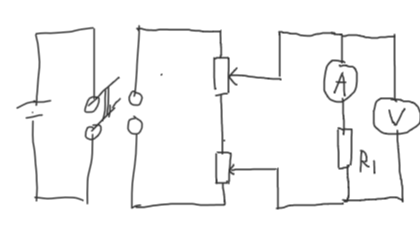
\includegraphics[scale=0.6]{R1}
			\centering
			\caption{测量R1伏安特性的电路图}
			\label{R1png}
		\end{figure}
		\begin{table}[htbp]
			\centering
			\caption{通过$R_1$电流与总电压的关系}
			\label{R1_relation}
			\begin{tabular}{ccccccccc}
				\toprule
				$U$/V & 0.100 & 0.201 & 0.297 & 0.410 & 0.520 & 0.631 & 0.742 & 0.864\\
				\midrule
				$I$/mA & 1.70 & 3.32 & 4.82 & 6.72 & 8.60 & 10.30 & 12.10 & 14.08\\
				\bottomrule
				\end{tabular}
		\end{table}
		\par 
		表\ref{R1_relation}中的$U$为电流表与待测电阻分得的电压之和这从图\ref{R1png}中的电路连接就可看出
		。根据上面的数据,我们可以做出伏安特性曲线。
		\begin{figure}[htbp]
			\includegraphics[scale=0.65]{R1_curve}
			\centering
			\caption{$R_1$的伏安特性曲线}
			\label{R1curve}
		\end{figure}
		\par 
		从图\ref{R1curve}中可以看出对于普通的电阻,通过其电流与其两端之间的电压呈现出很好的线性关系。根据
		线性拟合可以得到$I$随$U$的变化关系为:
		$$
		I = 16.24U + 0.0010
		$$
		从而可以计算出$R_1$的阻值为:
		$$
		R_1 = \frac{1}{16.24} \times{1000} - R_I = 52.5
		$$
		\subsubsection{$R_2$的测量}
		\begin{table}[htbp]
			\centering 
			\caption{使用多用电表测量待测电阻$R_2$的阻值}
			\begin{tabular}{ccc}
				\toprule
				$R_2^{'}/\Omega$ & $R_0/\Omega$ & $R_2/\Omega$ \\ 
				\midrule
				1002.6 & 0.2 & 1002.4\\
				\bottomrule
			\end{tabular}
			\label{R2_first}
		\end{table}
		\par 
		本次实验的电阻额定功率依然是0.25W,可以计算允许通过的最大电流大小为:
		$$
		I = \sqrt{\frac{P}{R}} = \sqrt{\frac{0.25}{52.84}} = 0.015
		$$
		\par 
		根据上面的计算得知在测量时不能使得通过$R_2$的电流大于15mA,因此给出如表\ref{expansion2}的电表量程
		选择:
		\begin{table}[htbp]
			\centering
			\caption{电表的量程选择}
			\label{expansion2}
			\begin{tabular}{ccc}
				\toprule
				& 量程 & 内阻\\
				\midrule
				电压表 & 3V & $600\Omega$\\
				电流表 & 3mA & $23.5\Omega$\\
				\bottomrule
			\end{tabular}
		\end{table}
		\par 
		显然,对于电阻阻值超过电压表内阻的情况,我们应选择电流表内接的测量方法,电路图与图\ref{R1png}一致
		。
		\begin{table}[htbp]
			\centering
			\caption{通过$R_2$电流与总电压的关系}
			\label{R2_relation}
			\begin{tabular}{ccccccccc}
				\toprule
				$U$/V & 0.290 & 0.500 & 0.798 & 1.200 & 1.628 & 1.992 & 2.388 & 2.810\\
				\midrule
				$I$/mA & 0.290 & 0.488 & 0.780 & 1.170 & 1.600 & 1.950 & 2.330 & 2.740\\
				\bottomrule
			\end{tabular}
		\end{table}
		\begin{figure}[htbp]
			\includegraphics[scale=0.65]{R1_curve}
			\centering
			\caption{$R_2$的伏安特性曲线}
			\label{R2curve}
		\end{figure}
		\par 
		从图\ref{R2curve}可以看出,电流随电压的变化呈现出很好的线性关系,通过线性拟合得到了$I$随$U$的变化
		关系:
		$$
		I = 0.9747U + 0.0078
		$$
		那么计算出$R_2$的真实电阻为:
		$$
		R_1 = \frac{1}{0.9747} \times{1000} - R_I = 1002
		$$
	\subsection{测定稳压二极管的伏安特性}
		\par 
		本次实验不再使用指针表,而是使用数字表,由于数字表测量电压时内阻可达10M$\Omega$,因此将其视为不导
		电是完全合理的,所以采用电流表外接的方法进行测量。首先给出二极管正向通电时的电压、电流数据。
		\begin{table}[htbp]
			\centering
			\caption{稳压二极管正向通电时电流随电压的变化关系}
			\label{diode_relation+}
			\begin{tabular}{cc|cc|cc}
				\toprule
				$U$/V & $I$/mA & $U$/V & $I$/mA & $U$/V & $I$/mA\\
				\midrule
				0.050 & 0.00 & 0.720 & 0.20 & 0.807 & 3.46 \\
				0.149 & 0.00 & 0.722 & 0.33 & 0.817 & 4.46 \\
				0.256 & 0.00 & 0.755 & 0.81 & 0.825 & 5.45 \\
				0.374 & 0.00 & 0.772 & 1.33 & 0.833 & 6.47 \\
				0.490 & 0.00 & 0.785 & 1.92 & 0.841 & 7.80 \\
				0.603 & 0.02 & 0.793 & 2.41 & 0.849 & 9.19 \\
				0.675 & 0.10 & 0.801 & 2.92 & 0.853 & 9.97 \\
				\bottomrule
			\end{tabular}
		\end{table}
		\par 
		从表\ref{diode_relation+}中容易看出,稳压二极管的伏安特性不是线性的,从正极到负极有一个明显的电势
		降落。下面给出稳压二极管正向通电时的伏安特性曲线。
		\begin{figure}[htbp]
			\centering
			\includegraphics[scale=0.65]{diode_curve+}
			\caption{稳压二极管正向通电的伏安特性曲线}
			\label{diode_curve+}
		\end{figure}
		\par 
		计算$U=0.8$V时的静态电阻值:
		$$
		R_D = \frac{U}{R} = \frac{0.801}{2.92} \times 1000 = 274
		$$
		\par 
		下面给出稳压二极管反接时的电压、电流数据:
		\begin{table}[htbp]
			\centering
			\caption{稳压二极管反向通电时电流随电压的变化关系}
			\label{diode_relation-}
			\begin{tabular}{cc|cc|cc}
				\toprule
				$U$/V & $I$/mA & $U$/V & $I$/mA & $U$/V & $I$/mA\\
				\midrule
				-0.540 &  0.00 & -5.169 & -3.00 & -5.215 & -10.10 \\
				-1.608 &  0.00 & -5.177 & -4.01 & -5.220 & -11.08 \\
				-2.512 &  0.00 & -5.184 & -5.01 & -5.225 & -12.00 \\
				-3.544 &  0.00 & -5.191 & -6.00 & -5.234 & -14.00 \\
				-4.564 & -0.01 & -5.197 & -7.00 & -5.244 & -16.03 \\
				-5.147 & -1.00 & -5.203 & -8.01 & -5.254 & -18.09 \\
				-5.160 & -2.00 & -5.209 & -8.97 & -5.262 & -19.93 \\
				\bottomrule
			\end{tabular}
		\end{table}
		\begin{figure}[htbp]
			\centering
			\includegraphics[scale=0.65]{diode_curve-}
			\caption{稳压二极管负向通电的伏安特性曲线}
			\label{diode_curve-}
		\end{figure}
		\par 
		根据表\ref{diode_relation-}中的数据可以计算出$I=-10$mA时的动态电阻:
		$$
		R_{D}^{'} = \frac{\mathrm{d}U}{\mathrm{d}I} \approx \frac{\Delta U}{\Delta I} = \frac{5.220-5.209}{11.80-8.97}=5.2
		$$
		\par 
		由上表的数据计算$U=-4.0\mathrm{mA}$时的静态电阻时,得到的结果为无穷大,在老师的提醒之下才发现实验
		中一直存在的一个错误,就是电流表量程的选择,实验中使用的时四位半的数字表,因此表
		\ref{diode_relation-}中电流的两位小数意味着测量电流的量程选择了$200\mathrm{mA}$,由于实验中电流
		不会超过$20\mathrm{mA}$,应该选择$20\mathrm{mA}$的量程。重新选择量程后测得$U=-4.000\mathrm{V}$
		时$I=0.004\mathrm{mA}$,可以计算的静态电阻为:
		$$
		R_D = \frac{U}{I} = 1.0\times 10^{6}
		$$
	\subsection{1000$\Omega$电阻与稳压二极管并联的反向伏安特性}
		\par 
		首先给出反向的电流与电压的数据:
		\begin{table}[htbp]
			\centering
			\caption{稳压二极管反向通电时电流随电压的变化关系}
			\label{diode&r_relation-}
			\begin{tabular}{cc|cc|cc}
				\toprule
				$U$/V & $I$/mA & $U$/V & $I$/mA & $U$/V & $I$/mA\\
				\midrule
				-0.135 & -0.135 & -2.439 & -2.436 & -5.129 & -5.464 \\
				-0.469 & -0.468 & -2.788 & -2.787 & -5.144 & -5.962 \\
				-0.749 & -0.748 & -3.308 & -3.309 & -5.153 & -6.516 \\
				-1.118 & -1.116 & -3.950 & -3.954 & -5.164 & -7.514 \\
				-1.498 & -1.496 & -4.259 & -4.269 & -5.171 & -8.386 \\
				-1.773 & -1.771 & -4.804 & -4.837 & -5.189 & -11.089 \\
				-2.167 & -2.165 & -5.084 & -5.236 & -5.205 & -14.021 \\
				\bottomrule
			\end{tabular}
		\end{table}
		\par 
		做出伏安特性曲线:
		\begin{figure}[htbp]
			\centering
			\includegraphics[scale=0.65]{diode&r_curve-}
			\caption{稳压二极管负向通电的伏安特性曲线}
			\label{diode&r_curve-}
		\end{figure}
	\section{\large{思考题}}
		\subsection{}
		\par
		Q:使用多用表($20\mathrm{k}\Omega$以上各档)测量二极管的正向电阻,为什么各档测量的数值不同?如果测量
		一个线性电阻,情况会怎样?
		\par
		A:多用电表测量电阻的原理是给待测原件两端加上电压,测量通过待测元件的电流值,从而计算得到待测元件的电
		阻,可以想象,为了更加精确地测量电阻,选择不同量程的欧姆档时很有可能加在元件两端的电压不同,量程越大
		,电压越大,由于二极管是一个非线性元件,因此选择不同的档位测量得到的阻值不相同。若测量线性元件,理论
		上得到的阻值应该相同,但是由于大量程必然会导致绝对误差的增大。
		\subsection{}
		\par 
		Q:测量正向伏安曲线时你采用了哪种电表接法,为什么?
		\par
		A:采用了电流表外接法,由于数字表的内阻极大,约为$10$M$\Omega$,在实验中的电压下,电流表的分度值根本
		无法测出通过电压表的电流,因此电压表对我们的实验测量不造成影响。\\
	\section{分析与讨论}
		\par 
		对比表\ref{R1_first}与后面扣除了电流表内阻的真实的$R_1$的阻值,两者已经非常接近,相对误差已在百分之
		一以下,由于此实验中使用的指针式电表一点也不接近理想电表,若不用它们的内阻修正结果,那会造成相当严重
		的偏差。如果不考虑电表内阻,那么对测量结果造成的偏差为系统误差,并不影响结果的精密度,只会影响准确度
		。(同样对比表\ref{R2_first}与后面扣除了电流表内阻的真实$R_2$)
		\par 
		实验中测得的静态电阻,反映了一个非线性元件在恒定状态下的电阻;由实验数据近似计算出来的动态电阻,反映
		了一个元件对于电路中电压(电流)变化的响应。如果一个元件在某一范围内动态电阻极大,那么就说明通过这个
		原件的电流在这个范围内几乎不受电压的影响,即这个元件有着一定能力的控制电流的能力,如果一个元件在某个
		范围内动态电阻极小,同样可以知道这个元件有着一定的稳压能力,实验中测量的稳压二极管就是这样一种情况,
		对比其$U=-4.0$V的静态电阻与$I=-10$mA时的动态电阻就可以清晰地看出这一点。
		
\end{document}